\documentclass[aspectratio=169]{beamer}
\usetheme{Madrid}
\usepackage[utf8]{inputenc}
\usepackage[T1]{fontenc}
\usepackage{tikz}
\usepackage{amssymb}
\usepackage{graphicx}
\setbeamertemplate{navigation symbols}{}
\setbeamercolor{title}{fg=white,bg=orange!85!red}
\setbeamercolor{frametitle}{fg=white,bg=orange!85!red}
\setbeamercolor{block title}{bg=orange!85!red!20,fg=black}
\setbeamercolor{block body}{bg=orange!85!red!8,fg=black}
\setbeamercolor{item}{fg=orange!85!red}
\setbeamercolor{itemize item}{fg=orange!85!red}
\setbeamertemplate{itemize item}[triangle]

\title{Web Story 2 — Organizing the Telling}
\subtitle{Functions — reusable, named pieces of story logic}
\author{ByteForge --- Grade 8 --- App Builder}
\date{}

\begin{document}

\begin{frame}
    \titlepage
\end{frame}

\begin{frame}{Today's Plan}
    \begin{itemize}
        \item Your First Story Function
        \item A Function That Changes State
        \item Two Functions, One Page
        \item[$\bigstar$] BOSS --- A Story Told By Functions
    \end{itemize}
\end{frame}

\begin{frame}{A function RETURNS a value — it doesn't display one}
    \large
    \begin{itemize}
        \item \texttt{describeItem()} hands back a string; a SEPARATE line decides what to do with it. Keeping "compute" and "display" as two different steps is what makes a function reusable.
    \end{itemize}
\end{frame}


\begin{frame}{A function can read AND change outside variables}
    \large
    \begin{itemize}
        \item \texttt{addItem()} reaches OUTSIDE itself to push onto \texttt{inventory}
        \item Functions aren't limited to only using their own parameters.
    \end{itemize}
\end{frame}


\begin{frame}{One function's result, another function's input}
    \large
    \begin{itemize}
        \item \texttt{canAfford()} returns true/false; \texttt{showResult()} takes THAT value and decides what to display
        \item Chaining functions builds complex behaviour from simple pieces.
    \end{itemize}

    \begin{center}
    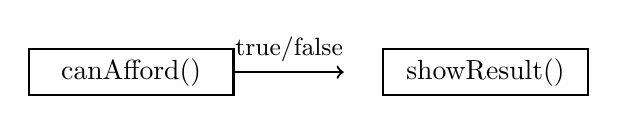
\begin{tikzpicture}[scale=0.9]

        \node[draw, thick, minimum width=2.6cm] (a) at (0,0) {canAfford()};
        \draw[->, thick] (a) -- (3,0) node[midway,above]{\small true/false};
        \node[draw, thick, minimum width=2.6cm] (b) at (5,0) {showResult()};
    \end{tikzpicture}
    \end{center}
\end{frame}


\begin{frame}{BOSS — a page organized entirely around functions}
    \large
    \begin{itemize}
        \item Splitting work into functions, each with ONE clear job, is what makes a real project readable, testable, and changeable later.
    \end{itemize}
\end{frame}

\begin{frame}{Real-World Examples}
    \large
    \begin{itemize}
        \item A recipe app's "calculateServings()" function reused across every recipe on the site is exactly this chapter's idea. Minecraft's real \texttt{/function} command (a named, reusable set of commands) works identically
        \item Define once, call from anywhere.
    \end{itemize}
\end{frame}


\begin{frame}{Image}
    \begin{center}
    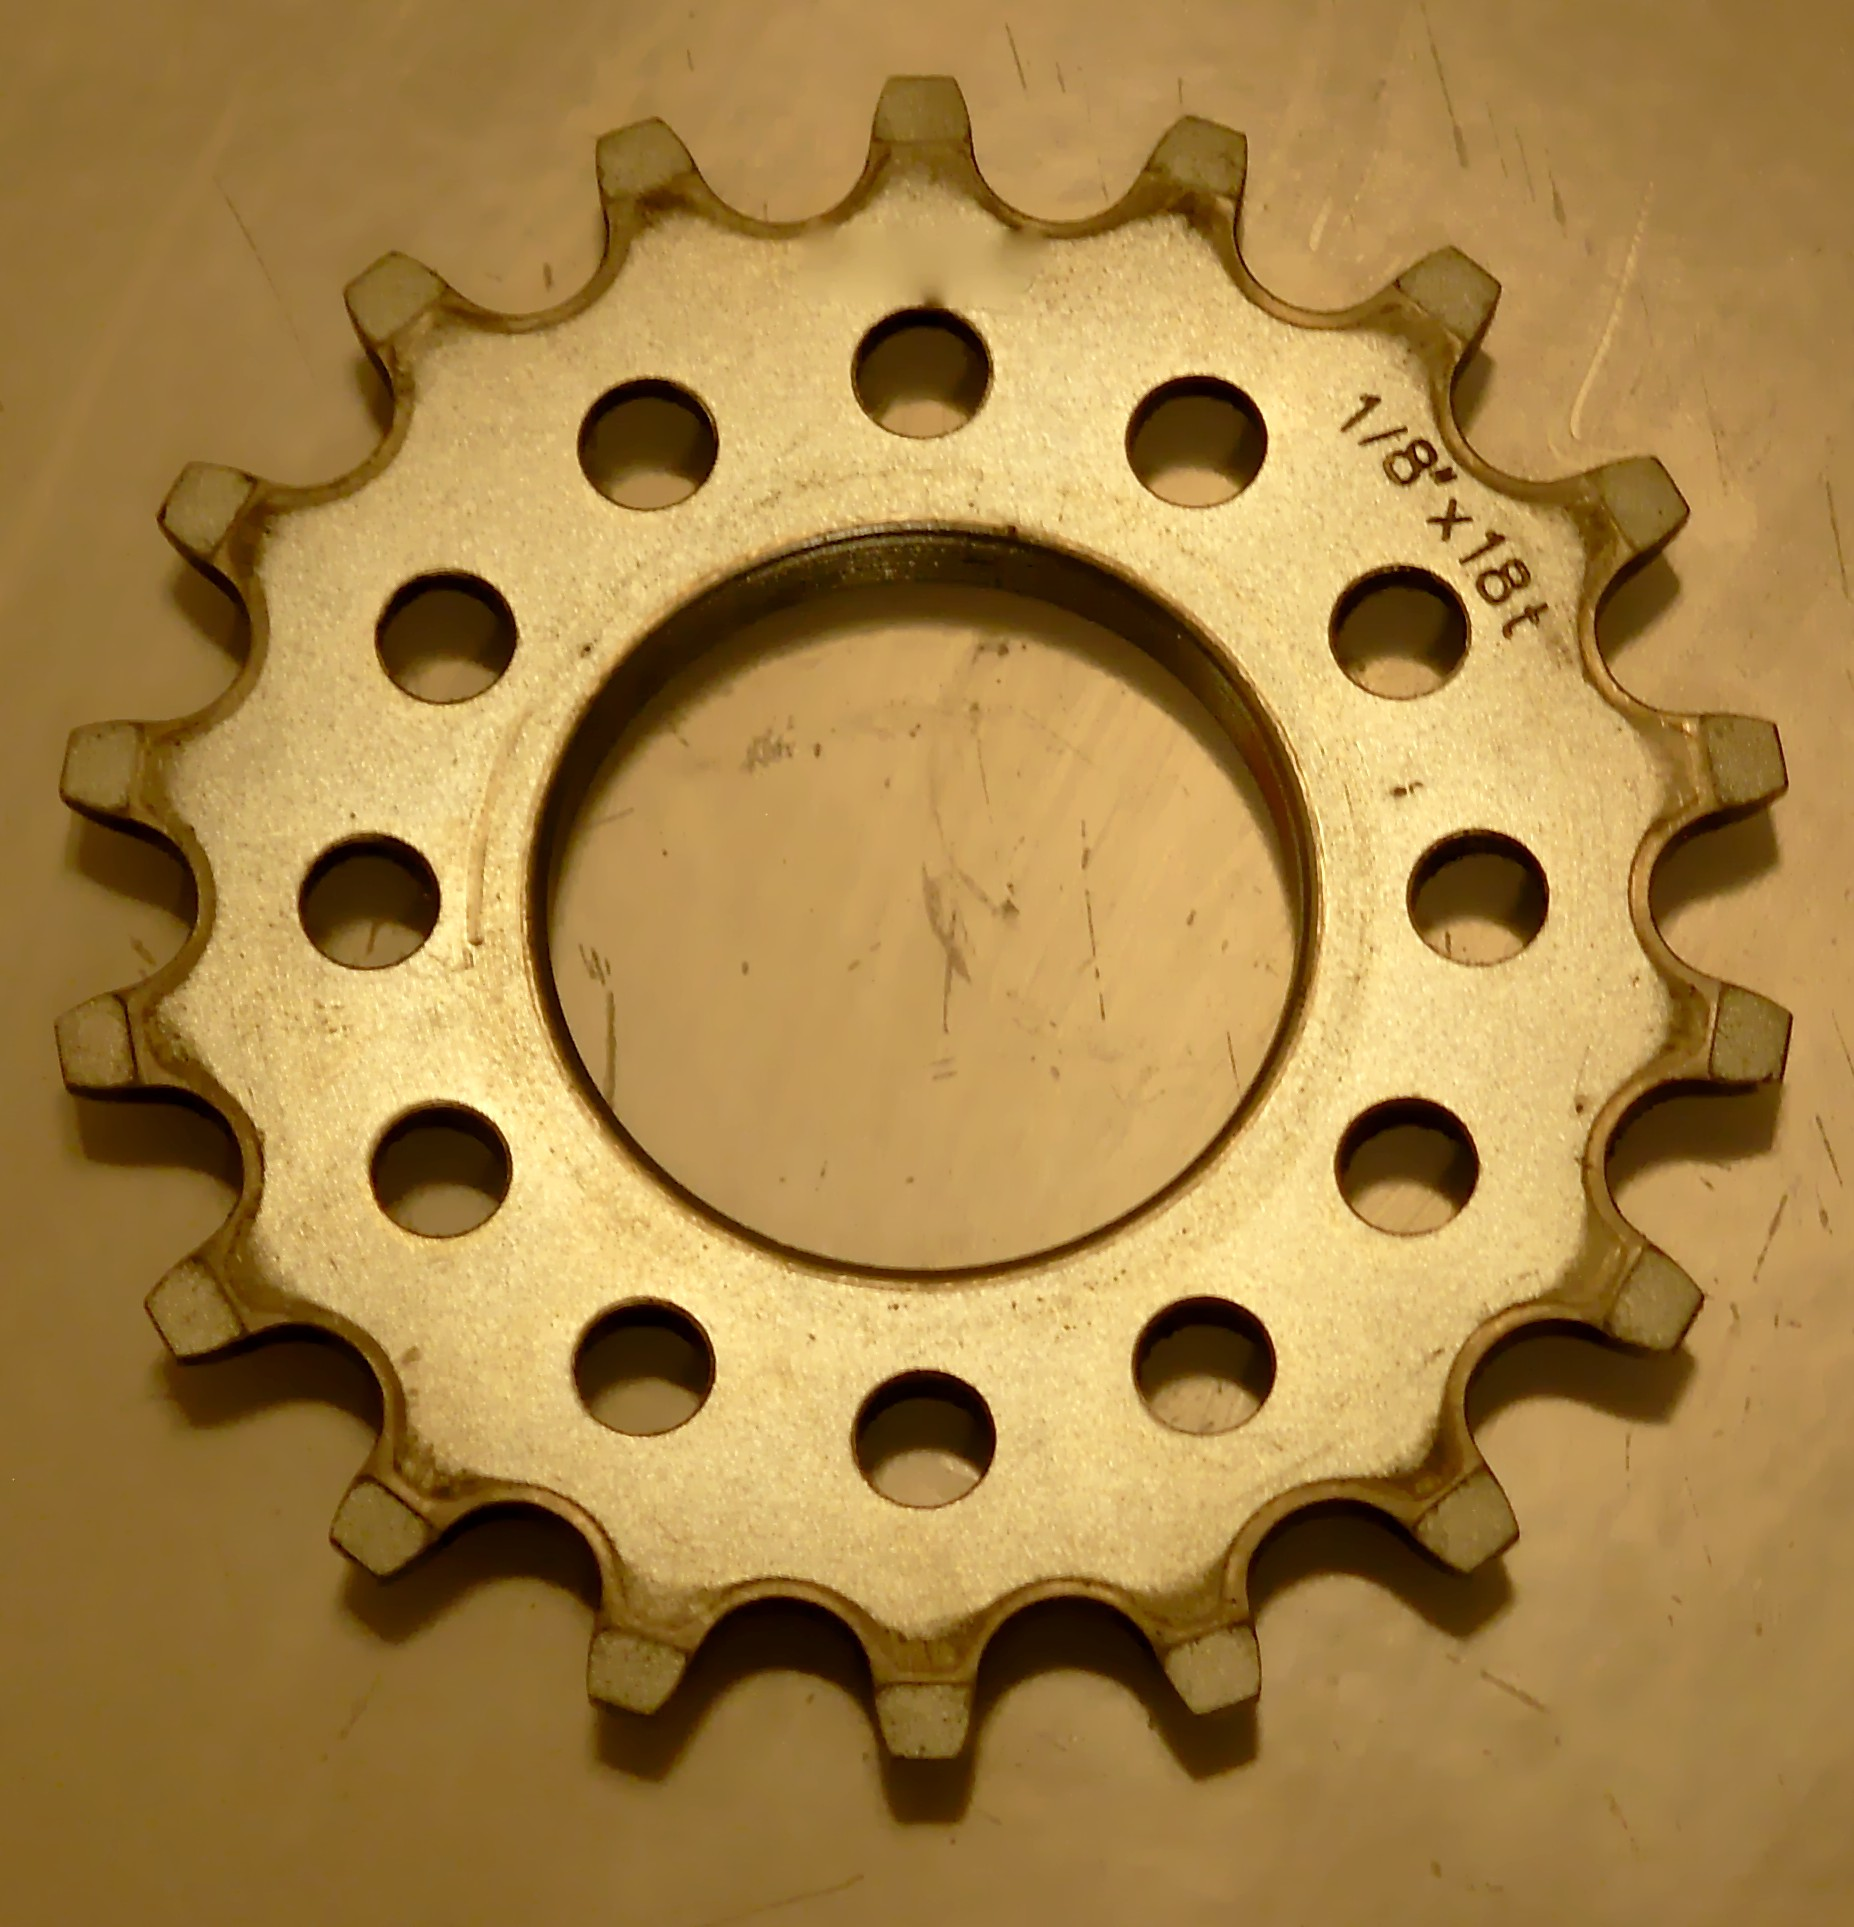
\includegraphics[width=0.5\textwidth]{images/gear.jpg}

    \large A function is defined once, does the same job every time it's called --- like a gear always doing the same defined turn.

    \small Fixed gear cog — John Reaves, public domain, via Wikimedia Commons
    \end{center}
\end{frame}

\begin{frame}{Let Them Discover}
    \Large
    Find one button in any app that clearly "computes something, then shows the result" (a checkout total, a BMI calculator). Which part do you think is the function's return value, and which part is just display?
\end{frame}

\begin{frame}{Your Turn}
    \Large
    Open the student map, find \textbf{Web Story 2 — Organizing the Telling}, and work through it
    hands-on --- everything you just saw, they now do themselves.
\end{frame}

\end{document}
